% options:
% thesis=B bachelor's thesis
% thesis=M master's thesis
% czech thesis in Czech language
% english thesis in English language
% hidelinks remove colour boxes around hyperlinks

\documentclass[thesis=B,english]{FITthesis}[2012/10/20]

\usepackage[utf8]{inputenc} % LaTeX source encoded as UTF-8
% \usepackage[latin2]{inputenc} % LaTeX source encoded as ISO-8859-2
% \usepackage[cp1250]{inputenc} % LaTeX source encoded as Windows-1250

\usepackage{graphicx}
 %graphics files inclusion
% \usepackage{subfig} %subfigures
\usepackage{amsmath} %advanced maths
\usepackage{amssymb} %additional math symbols
% \usepackage{algpseudocode}
% \usepackage{algorithm}
% \usepackage{algorithmicx}
\usepackage[ruled,vlined,linesnumbered]{algorithm2e}
\usepackage{dirtree} %directory tree visualisation
% % list of acronyms
\usepackage[acronym,nonumberlist,toc,numberedsection=autolabel]{glossaries}
% \iflanguage{czech}{\renewcommand*{\acronymname}{Seznam pou{\v z}it{\' y}ch zkratek}}{}
\makeglossaries

\newcounter{eqn}
\renewcommand*{\theeqn}{\alph{eqn})}
\newcommand{\num}{\refstepcounter{eqn}\text{\theeqn}\;}

\makeatletter
\newcommand{\putindeepbox}[2][0.7\baselineskip]{{%
    \setbox0=\hbox{#2}%
    \setbox0=\vbox{\noindent\hsize=\wd0\unhbox0}
    \@tempdima=\dp0
    \advance\@tempdima by \ht0
    \advance\@tempdima by -#1\relax
    \dp0=\@tempdima
    \ht0=#1\relax
    \box0
}}
\makeatother


% % % % % % % % % % % % % % % % % % % % % % % % % % % % % % 
% EDIT THIS
% % % % % % % % % % % % % % % % % % % % % % % % % % % % % % 

\department{Department of Computer Science}
\title{Application of Random Decision Forests in Astroinformatics}
\authorGN{Andrej} %author's given name/names
\authorFN{Pali{\v c}ka} %author's surname
\author{Andrej Pali{\v c}ka} %author's name without academic degrees
\authorWithDegrees{Andrej Pali{\v c}ka} %author's name with academic degrees
\supervisor{RNDr. Petr {\v S}koda, CSc.}
\acknowledgements{THANKS}
\abstractEN{In this bachelor's thesis we examine a machine learning algorithm called the Random Decision Forest and its usability on capabilities on astronomical problems. We present overview of existing implementations and algorithms that are suitable for Big Data. We wrapped several implementations of RDF into one self-contained package, that can be run with a single command. We conducted experiments that on both classification and regression problems and compared the results with other data mining algorithms. The experiments were performed on some well known data sets from the UCI repository and on some astrophysical problems, particularly spectra classification. The outcomes of the experiments show very promising results.}
\abstractCS{V n{\v e}kolika v{\v e}t{\' a}ch shr{\v n}te obsah a p{\v r}{\' i}nos t{\' e}to pr{\' a}ce v {\v c}esk{\' e}m jazyce.}
\placeForDeclarationOfAuthenticity{Prague}
\keywordsCS{rozhodovacie stromy, rozhodovacie lesy, data mining, astroinformatika}
\keywordsEN{decsion trees, decision forests, data mining, astroinformatics}
\declarationOfAuthenticityOption{4} %select as appropriate, according to the desired license


\begin{document}

% \newacronym{CVUT}{{\v C}VUT}{{\v C}esk{\' e} vysok{\' e} u{\v c}en{\' i} technick{\' e} v Praze}
% \newacronym{FIT}{FIT}{Fakulta informa{\v c}n{\' i}ch technologi{\' i}}

\setsecnumdepth{part}
\chapter{Introduction}
Machine learning has become phenomenon in recent years. Many businesses, institutes or organizations are increasingly more dependent on getting knowledge from data they managed to gather through their endeavors. One field that could highly benefit from machine learning approach is astroinformatics.  Astronomical surveys generate terabyres of high dimensional data in one session. However, conventional data mining algorithms fail on these kinds of data both in accuracy and in performance. 

Random Decision Forest \cite{BR01} was shown to be a very effective algorithm on data, that contain large amount of features. In this thesis we attempt to make a survey of available RDF algorithms and implementations that perform well on big data. We will perform tests both on datasets in the UCI repository \footnote{\url{http://archive.ics.uci.edu/ml/}} and on astronomical data.

We introduce common data mining and machine learning concepts and techniques in chapter~\ref{chap:DM}. Chapter~\ref{chap:DT} discusses the basic block of the RDF: the decission trees. Since some distributed RDF algorithms require parallel tree building process we also examine some scallable approaches to induction of decision trees. Chapter~\ref{chap:RDF} defines the RDF, examines some of their properties, and provides examples of both serial and parallel implementations of the algorithm. We implemented a wrapper that binds several Random Forest implementations together. We include a description of the wrapper in chapter~\ref{chap:wrapper}. In chapter~\ref{chap:Experiments} we show results from our experiments with the Random Forest model on astronomical data as well as some common datasets.
\setsecnumdepth{all}

\chapter{Knowledge discovery and data mining}
\label{chap:DM}
Knowledge discovery from databases (KDD) is an interactive and iterative ``process of identifying valid, novel, potentially useful, and ultimately understandable patterns in data'' \cite{andrassyova1999knowledge,Fayyad96thekdd}. Data mining (DM) is usually defined as a process where ``intelligent methods are applied to extract data patterns'' \cite{han2006data} and is merely a step in the process of KDD, however these two terms are often used synonymically. The KDD consists of these steps \cite{han2006data}:
\begin{description}
	\item[Data cleaning:] removing noise and incorrect data
	\item[Data integration:] combination of diferent data sources
	\item[Data selection:] selection of relevant data
	\item[Data transformation:] transformation of data into a format that is suitable for data mining
	\item[Data mining:] applying DM algorithms
	\item[Pattern evaluation:] evaluating the patterns that the DM process extracted and selecting those, that are relevant for our goal
	\item[Knowledge presentation:] transforming of extracted knowledge into a form that a user can understand
\end{description}

Data mining process involves building models based on some data. These models then help to extract patterns and relationships that are hidden inside the data. DM algorithms consist of a mix of three components \cite{Fayyad96thekdd}:
\begin{description}
\item [The model:] The model consists of a function and a representational form. The function determines what the model will do, e.g. classification or regression. The representational form means how the model will represent the data, e.g. a decision tree or a density function. The model contains parameters that are determined from the data.
\item [The preference criterion:] it computes a quality of model and helps to choose the model over others. It is usually a goodness-of-fit function of the model to the data.
\item [The search algorithm:] The function used when the model is constructed and fitted to the data.
\end{description}

This thesis concerns itself with a model that is represented in the form of a decision forest with both classification and regression function. The serach algorithms are some heuristic functions and a preference criterion a generalization error.

\section{Data mining methods}
A machine learning algorithm tries to learn a certain function that either describes the data in some way, or tries to predict an outcome. We recognize these basic methods of data mining \cite{fayyad1996data}:
\begin{description}
\item [Classification] This method maps the data set to a known finite set containing the labels. An example of classification is a model that decides whether a certain email message is a spam or not.
\item [Regression:] This method tries to predict a value of some numeric variable. An example of a regression may be prediction of redshifts based from the spectra.
\item [Clustering:] This method describes the data and tries to find a previously unknown finite set of categories the data would fall in. These categories can overlap each other, if certain data belong to multiple categories. An example of clustering may be discovering kinds of stars from spectra.
\item [Summarization:] This method attempts to find a compact description of data. It may simply mean calculating some statistical properties like means for each field, or it could mean something more complex, like discovering functional relationships between attributes.
\item [Dependency modeling:] This method tries to find dependencies between variables. 
\item [Change and deviation detection:] This method detects data, that are in some way different than previously measured data. This includes finding outliers, which are data that are in some way different from the majority. It is useful for finding data that are worthy of further examination.
\end{description}

A learning can either be supervised or nonsupervised. A supervised learning means, that we have a training data set, where the relationships between variables and their outcomes are already known. These data sets usually come either from historical data (such as weather patterns), or were labeled by humans specifically for the purpose of serving as a testing set. This can however bring bias and noise to the set. An unsupervised learning means, that the model is built from the data, that were not evaluated by anyone and where the relationships are unknown. The model has to discover these relationships and their possible outcomes by itself.

\section{Data set}
A data set is a collection of data. It is mostly represented as a table, where each column represents a variable and each row represents a member of the data set. A member of the data set is again a collection of values that represent its respective variable. A variable may be either categorical (discrete), or numerical (continuous).
\chapter{Decision trees}
\label{chap:DT}
		Decision trees are a group of supervised data mining methods, that use a tree-like structure to analyze data. They can perform either a classification of data, or a regression of data. The inner nodes of a decision tree represent testing on input attributes. \cite{CMP07} Terminal nodes in a classification tree represent the possible classes of tested objects. In a regression tree they represent predicted values for a given branch. Terminal nodes can either contain single values, or a probability vector of values \cite{TOP_DOWN_INDUCTION_SURVEY}. 

		The process of growing the decision tree is called an induction. Induction of an ideal decision tree is known to be NP-complete \cite{NP-COMPLETE}, so we have to use a heuristical approach for real-world applications. The induction consists of selecting the training data set, determining the splits at each nodes, choosing a stopping criterion and pruning of the tree. The methods we choose to perform these processes with, directly affect the performance of the tree. 

		Traditionally \cite{CART,C45-NUMERICAL}, the induction of a DT is performed in a recursive fashion, which is fine for small data, but tends to fail on big data problems. Therefore algorithms that are designed for big data use breadth-first approach \cite{mehta1996sliq,ben2010streaming}.

		\section{Choosing the sample}
			There are several approaches to choosing the training and testing sample. The simplest method is to just choose a fraction of the data as a training set and leave the rest for testing the tree. 
		
		\section{Splitting the nodes}
			Splitting is generally the costliest and most important phase of the induction. For each internal node, the inductor examines the input attributes in attempt to find the best split, i.e. at least one attribute, upon which it would branch the node. 

			An attribute may be either categorical (discrete) or numerical (continuous). Evaluating categorical attributes is generally straightforward, the easiest solution is to just create a branch for each possible value. A more complex one is to group several values together and creating a branch for each. We can use this to create binary decision trees.

			Additional steps must be taken when dealing with numerical attributes \cite{C45-NUMERICAL}.	 In this case the node is branched based on some threshold value or values which we need to find. At first, the data must be sorted based on the attribute. We'll mark those sorted values as \(\{v_1..v_m\}\). Each value \(v_i\) is then used as a dicrete value by the splitting criteria to determine the best split between two values \(v_i\) and \(v_{i+1}\). Evaluating numerical attributes is much more costly that the evaluation of categorical attributes due to the need of sorting.

			To determine how to split the nodes in the tree, we need to evaluate splitting criteria. There are essentially two types of splitting criteria:
			\begin{itemize}
			\item Univariate
			\item Multivariate
			\end{itemize}
			The univariate splitting criteria split the node according to the value of one attribute, while the multivariate criteria split the node on multiple attributes.

			\subsection{Univariate criteria}
				There are several categories of univariate criteria, such as impurity-based, normalized impurity-based or binary criteria. \cite{DMWithDecisionTrees}
				\subsubsection{Impurity-based criteria}
				Impurity-based criteria use an impurity measure, which is a function \(\phi\lbrack0,1\rbrack^k->R\). It for input \(P\), \(\phi(P)\) satisfies the following conditions:
				\begin{enumerate}
				\item \(\phi(P) \geq 0\)
				\item It is minimum if \(\exists i\) such that \(p_i = 1\)
				\item It is maximum if \(\forall i, 1 \leq i \leq k, p_i = 1/k\)
				\item It is symmetric with respect to components of P.
				\item It is smooth (differentiable everywhere) in its range.	
				\end{enumerate}
				The goodness-of-split due to discrete attribute \(a_i\) is defined as reduction in impurity of the target attribute after partitioning \(S\) according to the values \(v_{i,j} \in \textit{dom}(a_i)\):
				\[
					\Delta\phi(a_i,S)=\phi(P_y(S))-\sum\limits_{j=1}^{|\textit{dom}(a_i)|}{\frac{|\sigma_{a_i}=v_{i,j}S|}{|S|}*\phi\left(P_y\left(\sigma_{a_i}=v_{i,j}S\right)\right)}
				\]

				\paragraph*{Information Gain}
				Information gain is an  impurity-based selection. It uses an entropy of the input attributes as the impurity measure. The entropy of a set D is defined as:
				\[
				\textit{Entropy}\left(y, S\right) = \sum _{c_j \in \textit{dom(y)}}-\frac{|\sigma_{y=c_j}S|}{|S|}*\log_2\frac{|\sigma_{y=c_j}S|}{|S|}
				\] 
				Because of the attributes of the entropy, it tends to favor attributes with a lot of values. This can turn out to be problematic, if e.g. we'd include attributes that are unique for each specimen, such as an ID. \cite{ENSEMBLE}
				
				This can be remedied by using a gain ratio instead. It normalizes the information gain against the number of values of the feature.
				\paragraph*{Gini index}
				The Gini index is an impurity-based criteria that measures the divergences between the probability distributions of the target attributes values \cite{DMWithDecisionTrees}. It was popularized by the CART algorithm \cite{CART}. It is defined as follows:
				\[
					\textit{Gini}\left(y, S\right)=1 - \sum _{c_j \in \textit{dom(y)}}\left(\frac{|\sigma_{y=c_j}S|}{|S|}\right)^2
				\]
				\subsubsection{Binary criteria}
				Binary criteria are used to create binary trees. Binary criteria divide the domain of the input attribute into two subdomains. Let \(\beta(a_i, d_1, d_2, S)\) be a binary criterion value for attribute \(a_i\) over the data set \(S\) that divides it into two mutually exclusive and exhaustive subdomains \(d_1\) and \(d_2\). The binary criterion attemps to find the maximum value for the split, while satisfying the conditions for \(d_1\) and \(d_2\). An example of binary criterion is a twoing criterion. It was suggested in \cite{CART} after discovering that the Gini index performs badly when encountering wide domains. The twoing criterion is defined as
				\begin{multline}
					\textit{twoing}(a_i, S, d_1, d_2) = 0.25 * \frac{|\sigma_{a_{i} \in d_1}S|}{|S|}* \frac{|\sigma_{a_{i} \in d_2}S|}{|S|}  * \\ \left(\sum_{c_{1}\in\textit{dom}(y)}{
					\left|
					\frac{\left|
							\sigma_{a_{i}\in d_{1} \wedge y=c_i}S
						\right|}
						{|\sigma_{a_{i} \in d_1}S|} - \frac{\left|
							\sigma_{a_{i}\in d_{2} \wedge y=c_i}S
						\right|}
						{|\sigma_{a_{i} \in d_2}S|}
					\right|
					}\right)^2
				\end{multline}
				\subsubsection{Regression criteria}

				We have to use different criteria in regression, because we are dealing with continuous target values, instead of discrete. An example of criterion that is used for regression is minimization of a \textit{mean-square error}. It minimizes the square of the error between what is predicted and what should be the actual result. It is defined as:
				\[
					\textit{MSE}\left(y, \textit{pred}\right)= \frac{1}{|dom(y)|}*\sum _{c_j \in \textit{dom(y)}}\left(c_j - \textit{pred}\right)^2
				\]

		\subsection{Multivariate criteria}
			Although multivariate criteria are more effective than univariate, they are much more difficult to implement. They are usually based around finding the best linear combination of the attributes. Methods for finding this combination include:
			\begin{itemize}
				\item Neural trees \cite{NTrees}
				\item Hill climbing \cite{CART}
				\item Linear programming
			\end{itemize}

		\section{Stopping criteria and pruning}
			Stopping criteria tell the inducer when to stop splitting the nodes. Upon fullfilling the stopping criteria, the node is assigned the output label instead of splitting. There are various conditions and their combinations that can be used as the criteria, such as reaching the maximum tree depth, not gaining any significant information from the splitting criteria or not having enough cases in nodes. Choosing right stopping criteria is vital for the tree, because choosing very strict criteria may lead to an underfit tree. Making the criteria too benevolent, however, leads to overfitting the tree and losing information about the relationship between various attributes. To provide a solution, \cite{CART} introduced a pruning algorithm, that allows the tree to overfit and then prunes it to remove branches that cause the tree to lose generality.
				
		\subsection{Pruning}
		\label{sec:pruning}
				\paragraph*{Cost-complexity pruning}

				This is a pruning method suggested by \cite{CART}. The pruning is executed in two phases. In the first phase, we produce a sequence of trees \(T_0, T_1, T_2, \dots, T_k \), were \(T_0\) is the initial unpruned tree obtained by the induction and \(T_k\) is a tree consisting only of the root node. Each tree is obtained by replacing one or more subtrees in its predecessor by leaves. To determine which subtree to remove, we calculate an increase in error rate per pruned leaf by 
				\[\alpha = \frac{\mathrm{err(pruned(}T,t\mathrm{)},S\mathrm{)} - \mathrm{err(}T,S\mathrm{)}}{|\mathrm{leaves(}T\mathrm{)}|-|\mathrm{leaves(}\mathrm{err(pruned(}T,t\mathrm{)}\mathrm{)}|}\]
				where \emph{err} is an error rate for given tree \(T\) and set \(S\), \emph{pruned} is a pruned tree from \(T\) without subtree \(t\) and \emph{leaves} is a number of leaves in \(T\).

				In the second phase, we compute the generalization error for each tree \(T_i\), and select the tree with the lowest error

				\paragraph*{Reduced-Error Pruning}

				This method was introduced by \cite{Quinlan1987221}. We perform a test run on the original tree and check for each non-leaf node, whether replacing it with the most common class would reduce the error rate. This process continues, until we cannot reduce the error rate any more.

		\section{Testing the data}
		Once the tree induction process is complete, we can begin with testing the unknown data. Beginning at the root node, each entry from the data is tested based on the attributes the node represents and then passed into the subtree, where the process repeats itself. Once it reaches the leaf node, it is assigned the class that is in the node.
		
		\section{Decision trees algorithms}

			A general decision tree induction algorithm usually looks like this:

			\begin{algorithm}[H]
			\caption{BuildTree}
			\SetAlgoLined
			\KwData{
			\begin{itemize}
			\item dataset $S$
			\item features vector $X$
			\item output class $Y$
			\end{itemize}
			}
			\KwOut{tree $T$}
			\Begin
			{
			\If{stopping criterion}{
				return
			}
			\ForEach{$x$ in $X$} {
				compute gain from splitting on $x$
				\If{computed gain is the largest so far} {
					save the attribute
				}
			}
			Split on the attribute with the largest gain
			Apply recursively on each node gained by the split
			return current node
			}
			\end{algorithm}

			\paragraph*{ID3} It is a very simple decision tree algorithm proposed by Quinlan in \cite{INDUCTIONOFDT}. It uses information gain as a splitting criterion. The induction stops either when all the data belong to a single value, or when the information gain is less or equal to zero. The algorithm fails on missing attributes and cannot handle numerical attributes. It does not perform pruning.

			\paragraph*{C4.5} An improved version of the ID3 algorithm \cite{C45-NUMERICAL} that solves many of its problems. Instead of the information gain, it uses a gain ratio. The algorithm performs error-based pruning, handles missing values through corrected gain ratio criteria and can induce from data sets that contain numeric attributes. The inducing stops when the number of instances to be split is below certain threshold. Both ID3 and C4.5 cannot handle target labels that contain continuous values.

			\paragraph*{CART} Introduced in \cite{CART}. CART produces binary trees. What makes this algorithm significant and useful is that it handles both continuous and discrete output features and thus is capable of both classification and regression. It uses twoing criteria for classification and cost-complexity pruning. For regression it tries to minimize the prediciton squared error. Users can enhance its accuracy by providing probability distribution \textit{a priori}, and it can consider missclassification cost.

		\section{Performance and scalability}
		Traditional approaches to induction do not scale well for big data. Since they are usually built in a recursive fashion and require the data to be in the memory all the time, the system may run out of memory \cite{SCALABLE_RDF}. Another issue that has to be solved is the evaluation of attributes. As mentioned, the evaluation of numerical attributes is quite costly, because it involves sorting of all the values and then finding the best split. Many scalable algorithms try to speed up this process by pre-sorting the data \cite{mehta1996sliq,shafer1996sprint}, while others try to first pre-process them, as is the case with SPDT, which builds histograms from those attributes\cite{ben2010streaming}. Splitting on discrete attributes, while easier than splitting on numerical attributes, is not without its own problems. Search for a good split involves searching through subsets of the whole set of possible attributes, which in naive implementation would include searching throug \(2^n\) possibilities, where \(n\) is the number of items in the set. Thus this also requires a quick algorithm \cite{mehta1996sliq}.

		To further overcome these limitations, we can parallelize the induction process, distributing it across several computing nodes. While this makes an implementation of the DT much more complicated, it allows for huge data sets, thus improving the accuracy of the tree.

		\subsection{Types of parallelism}
		There are several strategies for parallelization of DT using task parallelism, data parallelism or hybrid prallelism. \cite{PARALLEL_IMPLEMENTATION}
		\paragraph*{Task parallelism.} When using task parallelism, we distribute the decision nodes across several processors. The induction process starts on a single processor, which then proceeds with the induction as in the serial approach. When the number of decision nodes reaches the number of available processors, they are distributed among them. Then, each processor continues in the induction of the subtree with the assigned node as its root. The subtrees are then merged together as they are completed. An example of this approach is a parallel implementation of C4.5 algorithm in \cite{PARALLEL_INDUCTION}. 

		This approach has its disadvantages. The load on each processor is imbalanced, because each subtree can take considerabely different time to construct. This could be countered by splitting the subtrees further, after some processor finished its task. Moreover, each processor needs to have access to the full data set, meaning it either has to be copied to each processor, or the processors have to access it from a central location, creating a great amount of communication. 

		\paragraph*{Data parallelism.} In data parallelism, the data, instead of the tree nodes, are split among the processors. The processors construct each node together, locally evaluating the data they were assigned. Because the processors have to communicate and share their split evaluations each time a new node is created the data parallelism generates a lot of communication on the network. The data can either be split vertically or horizontally. 

		In a vertical split, each processor receives every record and its label, but only a distinct set of input attributes. When deciding where to split, it takes into account only the set of attributes it received. Each processor supplies the best split from its local attributes. From these local splits the best one is picked. The vertical split strategy can still suffer from load imbalance, because continuous attributes usually take longer to evaluate.

		When using a horizontal split, each processor is assigned a distinct set of the records, but with full set of attributes. Each processor then examines possible splits based on the data it received and then communicates its findings with the other processors. They then work together to find the best global split.

		\paragraph*{Hybrid parallelism.} This is a combination of the data and task parallelism. It tries to combine the low communication overhead of the task parallelism with the lower memory requirements and processing amount of the data parallelism. The nodes that would have to cover large amount of examples use data parallelism to lower the load balance of each node. On the other hand, nodes, that cover few examples can be effectively distributed among several processors without significant memory overhead and thus eliminating costly interprocessor communication.

		\subsection{Examples of parallel DT algorithms}
			\paragraph*{SLIQ} It is a decision tree algorithm, that handles both numerical and categorical data \cite{mehta1996sliq}. In contrast with conventional decision tree algorithms which build tree recursively, SLIQ uses breadth-first tree growing strategy. To speed up numerical data, it pre-sorts the data set by each numerical attribute. 
			\paragraph*{SPDT}
			This algorithm solves the problem of storing all of the big data in one processor by using the horizontal data parallelism described above. Because the partitioned data may still be too big to be handled by each processor, the SLIQ build histograms of the records.

		\section{Advantages and disadvantages}
		As we can see, one of the main advantages of a DT is its simplicity and intuitiveness. They can be used on all sorts of data, both for classification and for regression. They allow for errors in data and, with some improvements, can handle missing values well \cite{DMWithDecisionTrees,CMP07}. Decision trees can be converted to a set of rules just by following branches from the root node to a leaf node. Some are capable of handling both numeric and categorical values and some algorithms can be used both for classification and regression.

		On the other hand, non-parallel decision trees do not perform well on high dimensional data. They are also sensitive to noise and irrelevant attributes and they easily overfit or underfit.
\chapter{Random Decision Forests and Random Ferns}
\label{chap:RDF}
	RDF is an ensemble classification method using \(K\) decision tree classifiers \({h(x, \Phi_k), k = 1\dots K} \), where \(x\) is the input data and \({\Phi_k}\) are independent identically distributed random vectors \cite{SELECTION_OF_DT}. The random vector \(\Phi_k\) represents the randomness that is injected into each DT and its nature and content is dependent on a concrete use. The randomness is usually introduced by randomly sampling the subset of input features and/or by bagging. After finishing the run in each tree, they vote for the final result, which will be chosen as the final class that will be assigned to that data entry.

	As with the Decision Trees, the performance of the RDF is directly affected by several factors such as the number of the trees, the means of introducing randomness into the induction, the voting process or the induction of the trees themselves.

	\section{Number of trees}
	It can be shown, that by adding more trees, the error rate does not increase or decrease infinitely, but converges to a limiting value. Suppose we have an ensemble of classifiers \(h_1(\textbf{x}), h_2(\textbf{x}),\dots,h_K(\textbf{x})\). Define function \(\textit{mg}(\mathbf{X},Y)\) as:
	\[\textit{mg}(\mathbf{X},Y)=\textit{avg}_kI(h_k(\mathbf{X})=Y)-\textit{max}I(h_k(\mathbf{X})=j)\] It gives an amount by which an average number of votes for the right class exceedes the average number of votes for any other class. 

	Define generalization error as \(PE^*=P_{\mathbf{X},Y}(\textit{mg}(\mathbf{X},Y) < 0)\). In decision forests, the above mentioned classifier \(h_k(\textbf{X})=h_k(X, \Phi_k)\). By applying the Strong Law of Large Numbers, we can conclude, that by increasing the number of trees, the generalization error \(PE^*\) of all sequences~of~\(h_1(\mathbf{X},\Phi_k)\), \(h_2(\mathbf{X}, \Phi_k)\),~\(\dots, h_K(\mathbf{X}, \Phi_k)\) almost surely converge to \cite{BR01}:
	\[
	P_{\mathbf{X},Y}(P_{\Phi}(h(\mathbf{X}, \Phi)=Y)-\textit{max}P_{\Phi}(h(\mathbf{X}, \Phi)=j))
	\]
	This implies that there is a threshold for the number of trees in the forest, above which the trees provide only small or nonexistent improvement to the accuracy \cite{SELECTION_OF_DT}. This of course does not mean that the forest has reached an optimal number of trees --- a subset of the trees usually provides much better results. To reduce the number of trees, we can prune the forest, not unlike we did with individual trees as described in section~\ref{sec:pruning} --- in RDF, we call this process the selection. To do this, we need to define selection criteria and selection method.

	Selection criteria divide into filters and wrappers. Filtering criteria select trees \textit{a priori}, not taking into account the combined accuracy of the subset. Wrapper criteria select trees \textit{a posteriori}, by optimizing the combined performance of the subset \cite{PRUNING_RDF}. Wrapper criteria are generally better for building optimized subset of classifiers out of an existing set. Methods of selection may be based on several approaches.
	One of the simplest methods usually use simple rules based upon some metric of individual classifiers. An example of these may be a method that would select \(n\) most accurate trees out of all, or select \(n\) most accurate trees for each class. These methods usually do not require much computational power, but since they do not explore different subsets of classifiers, they may not find the best suboptimal result \cite{PRUNING_RDF}. 
	
	A more advanced, but fast and simple methods are Sequential Forward Selection (SFS) and Sequential Backwards Selection (SBS). They both iteratively build sub-optimal subset of the ensemble by searching through the ensemble and selecting classifiers according to some given criterion. They differ in what they do after the selection. SFS starts with an empty set of classifiers and in each iteration, tests each tree and selects one, that would most improve the performance of the whole subset. SBS, on the other hand, starts with the full subset of the ensemble and at each step of the iteration, removes the classifier that drags the whole performance down the most. \cite{SELECTION_OF_DT} The proccess stops either when the accuracy of the subset reaches a certain threshold, or after a number of iterations \cite{DESIGNING-MULTIPLE-CLASS-SYS}. 

	\section{Bagging}
	One of the techniques that is used in the RDF is \textbf{b}ootstrap \textbf{agg}regat\textbf{ing}. For each sampled instance \(T_k\) of the training set \(T\), \(k = 1, 2, \dots, K \) we randomly sample a training set with replacement from the original training set. It has the same size as the original and because it was sampled with replacement, some of the instances may appear more than once, while some may be completely excluded. \cite{quinlan1996bagging}. During the induction the bagging is used in two ways. One is for the induction of the trees, where each tree is induced from a different sample. The second is to give ongoing estimates about the generalization error, strength, correlation or variable importance.

	The most common out-of-bag estimate is the estimate of the generalization error. Suppose we have a classifier \(h_k\) which was trained on the training set \(T_k\) sampled from \(T\). Then for each \(y,\mathbf{x}\) from the training set \(T\) we aggregate those classifiers, that do not contain the given instance and let those classifiers vote for the right results. The out-of-bag error rate is the average of error rates all such aggregate classifiers on the training set \cite{breiman1996out}.

	\section{Random Ferns}
	Random Ferns \cite{ozuysal2010fast,ozuysal2007fast} is an ensemble model inspired by Random Decision Forest, that uses structures called \emph{ferns} instead of trees for classification. Each contains a set of binary features that are considered to be independent of each other. Ferns classify using a Na\"{\i}ve Bayes Classifier with their respective set of features as a input feature vector.

	\subsection{Na\"{\i}ve and Semi-na\"{\i}ve Bayes Classification}
	Let \(c\) be a set of classes and let \(p\) be a set of binary input features. A Bayes Classifier attempts to find such a class \(c_i\), that the probability \(P(C=c_i|f_1,f_2,\dots,f_n)\) will be maximal. By applying the Bayes theorem we get: 
	\[
	P(C=c_i|f_1,f_2,\dots,f_n)=\frac{P(f_1,f_2,\dots,f_n|C=c_i)P(C=c_i)}{P(f_1,f_2,\dots,f_n)}
	\] 
	We can ignore the denominator, because it is constant for all \(c_i\) and only scales the result, and we also assume that \(P(C)\) has uniform distribution \cite{ozuysal2010fast}. The problem is then reduced to finding only the probability \(P(f_1,f_2,\dots,f_n|C=c_i)\). This is computationally infeasible, because it would require to compute \(2^N\) possibilities for each class. A Na\"{\i}ve Bayes Classification assumes, that all features in the set are totally independent from each other, which means that the equation 
	\[
		P(f_1,f_2,\dots,f_n|C=c_i)=\prod_{j=1}^{N} P(f_j|C=c_i)
	\]
	which removes the complexity constraint but almost always is not true. This deeply affects the accuracy of the classifier, because it ignores any kind of relationship between the features. To rectify this problem, Random Ferns uses approach called Semi-na\"{\i}ve Bayes Classification and groups features into \(M\) groups called \emph{ferns}. Each fern has size \(S=\frac{N}{M}\) and is defined as \(F_k=\left\{f_{\sigma(k,1)},f_{\sigma(k,2)}, \dots,f_{\sigma(k,S)}\right\}\), where \(\sigma_{k, l}\) is a random permutation function with a range \([1,N]\).

	Ferns can be considered to be simplified trees. To transform a tree to a fern we have to follow these steps:
	\begin{enumerate}
	\item Transform all non-binary features into binary
	\item Modify tree in such a way, that on each level, it will evaluate the same test.
	\item Remove the hierarchical structure of the tree, creating only a sequence of test to be performed.
	\end{enumerate}



	\section{RDF algorithms and implementations}
	The classic RDF algorithm, called Forest-RI was introduced by Breiman~in~\cite{BR01}. It serves as a basis for all the other random forest algorithms. It builds \(n\) trees using a modified CART algorithm, where each node is built using \(m\) randomly selected features. Breiman suggests using \(\lfloor \log_2|A|)+1\rfloor\) as the~number of~features, where \(A\) is the input features vector. Neither the trees nor the forest are pruned. The algorithm also computes an out of bag error and a confusion matrix. 

	\begin{algorithm}[H]
		\caption{FOREST-RI}
		\label{alg:forestri}
		\KwData{
		\begin{itemize}
		\item data set $S$ 
		\item feature vector $X$ 
		\item output class $Y$
		\item number of trees $N$
		\end{itemize}
		}
		\KwOut{a Random Forest classifier $F$}
		\Begin
		{
		\For{$i = 0$ to $N$} {
			$s,s_t$ = bag($S$)\\
			$x$ = choose random input vector of size $m$ from $X$\\
			$t$ = buildtree($s$, $x$, $Y$)\\
			add $t$ to $F$\\

		}
		return $F$
		}

	\end{algorithm}

	\subsection{Parallelization}
	The parallelization of both the induction and the testing is possible. Because the induction of the random forest is based on building of large amount of trees, it is very costly for data with millions of records and many dimensions. That makes the induction of decision forest a viable candidate for attempts on parallel implementation.

	One way to parallelize the induction process is to simply divide the process between the available processors.

	A popular approach to parallelization of the Random Forest is to use the MapReduce model \cite{SCALABLE_RDF,han2013scalable}. MapReduce is a programming model for parallel processing of large data sets across several processors  \cite{dean2008mapreduce}. One processor is designated to be a master and is assigned other processors, called workers. These work on problems assigned by the master. A MapReduce process has two basic steps:
	\begin{description}
	\item [Map:] In this step, the master divides the data among the workers and sends the data to them. Each worker can then either process the data, or become a master itself, divide the data again and send them to another set of workers, or process the data and send the partial result to the master.
	\item [Reduce:] The master combines and processes the data it received from the worker nodes during the Map step. This can either happen locally on the master processor, or it can again parallelize it and let the workers do it.
	\end{description}

	A naive approach to the induction of Random Forest in MapReduce would be to partition data across the workers and in the \emph{Map} function build the tree from the data block. The majority voting would take place in the \emph{Reduce} step. However, because the size of the data set may be too big even after partitioning a more clever way has to be taken.
	
	One possible approach \cite{SCALABLE_RDF} in implementing the Random Forest on MapReduce model is based on the SPDT algorithm \cite{ben2010streaming}. This algorithm generates \(K\) trees in a breadth-first fashion. It first partitions the training data set into data blocks and distributes them across the workers. Each worker receives a constant number of data blocks. The trees are built by bagging from all the records. The indices of samples used for the creation of the trees are stored in a bagging table, that contains a column for each tree. The table is also distributed to each worker.

	The induction runs in parallel on each worker. The trees are built breadth-first instead of recursivelly, which means that at each step of an iteration, one level of nodes is created for all the trees. 

	In the Map function, each worker calculates local histograms of features for each tree. It does so by iterating through the data set, checking each record agains the bagging table. If the column for the current tree contains the record, the histogram is updated from it. After all the workers finish the mapping procedure, they send a tuple of \((\textit{treeId}_k, \textit{hist}_k)\) back to the master. This process is described in algorithm \ref{alg:map}.

	\begin{algorithm}[H]
	\caption{Map step}
	\label{alg:map}
	\KwData{
	\begin{itemize}
		\item Training data set $D$ 
		\item forest model $F$ 
		\item and bagging table $T$
	\end{itemize}
	}
	\KwOut{a tuple of \((\textit{treeId}_k, \textit{hist}_k)\)}
	\Begin{
		\ForEach{record $d$ in $D$}
		{
			\ForEach{tree $k$ in $F$}
			{
				\If{$T$ contains $d$ for tree $k$ and tree $k$ is not fully grown }
				{
					update(\(\textit{hist}_k\), $d$)
				}
			}
		}

		\ForEach{tree $k$ in $F$}
		{
			Emit(\((\textit{treeID}_k, \textit{hist}_k)\))
		}
	}
	\end{algorithm} 

	The master then begins the \emph{Reduce} step, where each reducer receives all the histograms that belong to their respective tree. Reducers first merge their local histograms into a global histogram for one tree. Then for each node they either mark the node as leaf, if the stopping critera are met, or decide on a splitting point and split the node. They send back the newly created nodes along with the tree ID back to the master. After all the receivers finish their jobs, the master updates the forest with the newly created nodes. The process finishes after all trees are fully built. We provide a pseudocode of this process in algorithm \ref{alg:red}.

	\begin{algorithm}[H]
	\caption{Reduce step}
	\label{alg:red}

	\KwData{
	\begin{itemize}
		\item an ID of a tree \(k\) 
		\item \(V_k\), set of all histograms for the tree \(k\)
	\end{itemize}
	}
	\KwOut{List of splits for all the nodes in the current level for tree \(nodes\) \(k\)}
	\Begin{
		\(\textit{globalHistogram}_k\) = merge(\(V_k\))

		\ForEach{node $n$ in $k$}
		{
			\(\textit{nodeHist}\) = \(\textit{globalHistogram}_k(n)\)
			\(\textit{splitConditions}\) = calculateSplit(\(textit{nodeHist}\))
			\If{stopping critera(\(textit{nodeHist}\))}
			{
				\(\textit{nodes}_i\) = leaf(\(\textit{splitConditions}\))
			}
			\Else
			{
				\(\textit{nodes}_i\) = split(\(\textit{splitConditions}\))
			}			
		}
		Emit(\((\textit{treeID}_k, \textit{hist}_k)\))
	}
	\end{algorithm} 

	\subsubsection{Parallelization using the GPU}
	Modern GPUs are based on a massively parallel architecture, consisting of a high number of computing cores. Although these cores are usually slower than the ones used in a general purpose CPU the architecture of a GPU is designed to allow for a high throughtput and massive parallelism. Therefore, they may provide significant boost for applications that benefit from such a highly parallel environment, such as Random Decision Forests. However, there has not been much research done in this field, with only a few studies being published \cite{sharp2008implementing,grahn2011cudarf, liao2013learning}.
	
	\paragraph*{CUDA architecture overview:} There are two competing frameworks, that are used for a GPU programming: a proprietary CUDA \footnote{\url{http://www.nvidia.com/object/cuda_home_new.html}} from nVIDIA and OpenCL \footnote{\url{https://www.khronos.org/opencl/}}. We provide an overview of an implementation based on the CUDA technology \cite{grahn2011cudarf}. A CUDA enabled GPU consists of several cores, also called Shader Processors (SP). Each of these cores has its own private memory and registers. Eight SPs form a Streaming Multiprocessor (SM). This SM also has its own memory, shared between SPs belonging to the same SM. SMs together form a GPU, which has a global memory, texture memory and a constant memory. These memories are accessible from all the SPs. 

	A CUDA program has two kinds of code: the sequential code, that runs on a host CPU and a CUDA code, called a \emph{kernel}, that runs on the GPU. Before a kernel can be executed on a GPU, the required data has to be transfered to the unit. Each instance of a kernel runs on its own GPU thread. These threads are organized into blocks, which run on a SM and blocks into grids, which represent kernels.

	\paragraph*{Implementations:} An implementation of Random Decision Forests, called \textit{cudaRF}, was introduced in \cite{grahn2011cudarf}. In this implementation, each tree of the forest is built using one thread. Since it is impossible to use recursion in a CUDA kernel, the trees have to be built iteratively. The data reading and preprocessing has to be done on a CPU, the resulting arrays are then sent to the GPU. The host then launches kernel that builds trees on the GPU in parallel. The trees are then kept in the GPU memory for querying. The kernel also computes statistics about the forest, such as out-of-bag error or variable importance. The testing also happens in parallel, where each tree of the forest is assigned to a thread and votes on the instances.

	A more recent implementation, \textit{CudaTree} \cite{liao2013learning}, allows for breadth-first task parallelism and depth-first data parallelism, or their combination. In the depth-first mode each CUDA thread block processes a subset of the data set for each feature and determines the best split for each node. All the threads work on single node. In the breadth-first mode, a whole level of nodes is constructed in parallel. This implementation also supports a hybrid more. The induction first stars in a depth-first fashion, but after reaching a certain depth it switches over to breadth-first. 

	As we mentioned, one of the advantages of computing on a GPU is GPUs inherent massive throughtput and parallelism. A GPU is designed specifically to run hundreds or thousands of computational tasks at once. It however has its disadvantages: 
	\begin{itemize}
	\item The need to transfer the data from the CPU to the GPU --- this creates some overhead before the computation starts and may prove to be a bottleneck
	\item A limited memory --- as of 2014, the typical size of a memory of a GPU is around 1 or 2 gigabytes, with professional GPUs having more (4 - 6 GB). This is enough for smaller data sets, but it will be a problem when one tries to induct a forest for larger datasets. This can be solved by transfering data between CPU and GPU, but that would slow down the whole process.
	\item A GPU provides significant boost only when the task requires such massive parallelism. Because the data transfers between the CPU and GPU have some overhead and the GPU cores being slower than the CPU as well as design specifically for massive parallelism, the task needs to be designed and tweaked for it.
	\end{itemize}

	\subsubsection{Other platforms}

\chapter{Random Decision Forest wrapper}
\label{chap:wrapper}
To simplify the testing with various Random Decision Forest implementations in a computing environment, we developed a package, that wraps around these different implementations and libraries. The wrapper should accept a single parameter file, that defines parameters such as locations of data sets and actions to be performed on them, forest and tree configurations and others. It also had to be easily extensible, so that more implementations of the algorithm could be added over time. An additional requirement was, that it should accept datasets in a CSV format as well as in a binary table in a FITS format (see Appendix \ref{app:FITS}).

The wrapper itself is written in the Python language. The language was chosen, because it is a powerful scripting language with an easily understandable syntax and there is an implementation of Random Forests in Python \cite{scikit-learn}. We have used Python version 3, but because we wanted to have at least a limited support for implementations running on older versions, we tried to keep the core backwards-compatible.

\section{Included implementations}
\begin{description}
\item[H2O:] It is a machine learning framework developed specifically for Big Data. It implememts various machine learning models, such as Deep Learning, K-means or Random Decision Forests, in a scalable manner. It can form clouds with other H2O instances running on the same network or with their addresses specified in an input file. It is possible to communicate with an existing cloud using either its REST API, or through a R console. During the testing, the H2O platform showed favorable speed of the induction and accuracy of the model. This Random Forest implementation is implemented in two ways: a Single Node, where the forest is built only on a single computing node and a distributed version, where it is built in the entire cloud. We chose only the single node version for the wrapper, because the distributed version is still in beta version and missign some features.

One of the drawbacks is that is builds only in-memory models. They cannot be serialized and thus we can run tests only if the H2O instance, where the model was built, has not been shut down or restarted. The single node Random Forest is also missing a regression mode, which is however included in the distributed version.
\item[Scikit-learn:] This is a Python library, that contains various machine learning algorithms, as well as a number of supporting algorithms and methods for scoring, handling of data sets and others \cite{scikit-learn}. We have included this library, because it delivers high-quality implementations of algorithms and is highly regarded among machine learning community. The library supports parallelism only over shared memory and cannot be used for distributed computing.
\item [cudaTree:] An implementation of the Random Forest model running on the GPGPU platform CUDA. It is implemented in the Python language, using the \textit{PyCUDA} package as a means to communicate with the GPU. It supports similar interface as RDFs from the scikit-learn library, but with less features. Among the missing features are x-validation and out-of-bag score.
\end{description}

\section{Integrating libraries}
We defined two wrapper classes, that bridge the interface our wrapper is using with the interface of the implementations. To set a standard interface, we defined base classes \texttt{base\_wrapper} and \texttt{base\_forest}. 

The \texttt{base\_wrapper} class serves as a main gateway with the underlying implementation. It provides an interface to import data from a CSV file and train a forest. The \texttt{import\_data} method accepts a path to the file and a boolean flag that signals if the data have a header. After importing the file, it returns a key, that identifies the file to the wrapper. The \texttt{train\_forest} method serves for inducing a forest. It accepts a key to the data set as its argument and returns an instance of a subclass of a \texttt{base\_forest}. The \texttt{base\_forest} supports scoring on a testing set, prediction, and getting an out-of-bag scores. 

\section{Additional features}
The wrapper supports training of Random Forest models, their scoring and running predictions. It supports data sets in CSV format, and can convert data sets in FITS binary tables into one. It supports scoring through x-validation, out-of-bag score and scoring with a separate training and testing data set. It also supports preprocessing of the features of the spectra extracted from the FITS files by binning them by their wave length.

\subsection{FITS handling}
The FITS files contain the measured spectra in a binary table. Each FITS file corresponds to one measurement. The conversion process maps each column in the binary table to a column in a CSV file. However, because of noise and other factors, there can be small errors in wave lengths in each spectra. In practice, this would mean that the spectra would not be aligned horizontally. We need to perform data binning to deal with these errors. 

\paragraph*{Binning}
\label{sec:binning} 
A binning groups values, that are near each other to one bin, using a central value as a new one. It is an approximation of what the actual value may have been on a given wave length. As a result, it reduces the length of the feature vector. When done on multiple rows, we first determine the maximal first wave length, \textit{first\_max}, from the set and minimal last wave length, \textit{last\_min}, from the set. These will serve as the starting and ending points of the binned wave lengths. We then choose a difference \textit{step} between the individual wave lengths that will be in the binned data. Then, for each spectrum, we iterate over values between \textit{first\_max} and \textit{last\_min} with \textit{step}. For each record in the spectrum, we have to find the first that has a wave length greater than the wave length of the current bin, \textit{next\_x}. Then we approximate the intensity measured over that wave length by determining the relative position of the bin between the \textit{next\_x} and the previous wave length and multiplying the intensity on the previous wave length by it. 

\subsection{Model validation, scoring and testing}
\label{sub:wrapper_test}
We support scoring by separate train and test sets and a k-fold x-validation. If the implementation of the Random Forest supports it, we also provide interface for accessing the out-of-bag score and matrix. If the user did not provide any test set, but wishes to perform the scoring, we support separating the original training set into two separate sets with a ratio defined by the user. When the user requests an x-validation, the wrapper either uses the x-validation of the implementation, or if the implementation does not support it out-of-the-box, it uses a built-in implementation. When using the built-in implementation, the wrapper generates \(k\) pairs of training and testing files, from which models are built in turn. After an x-validation is done, the wrapper returns a mean of the vector generated by the x-validation process. This process however does not work on earlier Python versions older than version 3. This is because of the difference between handling strings in IO.  

\chapter{Experiments}
\label{chap:Experiments}
We explored the performance on classification and regression problems of both astronomical and common datasets used for machine learning. We used implementations of Random Forests that are included in the wrapper described in Chapter \ref{chap:wrapper}. We include results for various number of trees with different implementations. We also include a comparison with other supervised machine learning algorithms, namely k-NN, support vector machines and neural networks.
\section{Astronomical experiments}
We conducted two experiments on astronomical data. We measured the classification performance and speed of Random Forest on classification of Be stars spectra. We classified raw data, extracted from the FITS files  ``as they were'', and then with various preprocessing transformations applied, such as binning and feature extraction \cite{bromovabeclass}. For a regression experiments, we chose the standard problem of predicting redshifts. It is a well known problem \cite{RED13,RED10,RED07} that is commonly used for benchmarking regressive machine learning algorithms.

\subsection{Spectra classification}
In this experiment, we tested the performance of Random Forests on Be stars spectra classification. Be stars are ``hot, rapidly rotating B-type stars with equatorial gaseous disk producing prominent emission $H_\alpha$ lines in their spectrum.''\cite{bromovabeclass} Their emission lines come essentially in these different shapes:
\begin{itemize}
\item a pure emission (Figure \ref{fig:pure_emission})
\item an emission with a small absorbtion (Figure \ref{fig:small_abs})
\item an emission with a large absorbtion (Figure \ref{fig:large_abs})
\end{itemize}

\begin{figure}

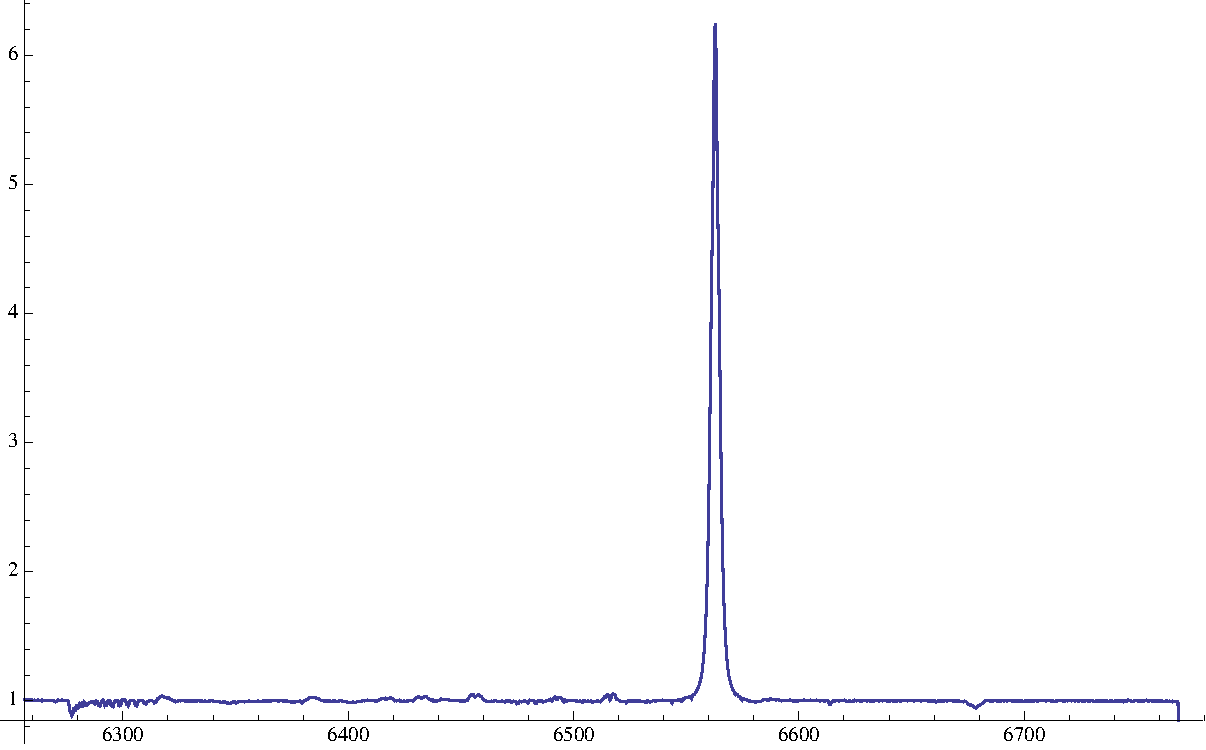
\includegraphics[width=300pt]{emission_spectrum}
\centering
\caption{Example of a pure emission spectrum}
\label{fig:pure_emission}

\end{figure}

\begin{figure}
\centering
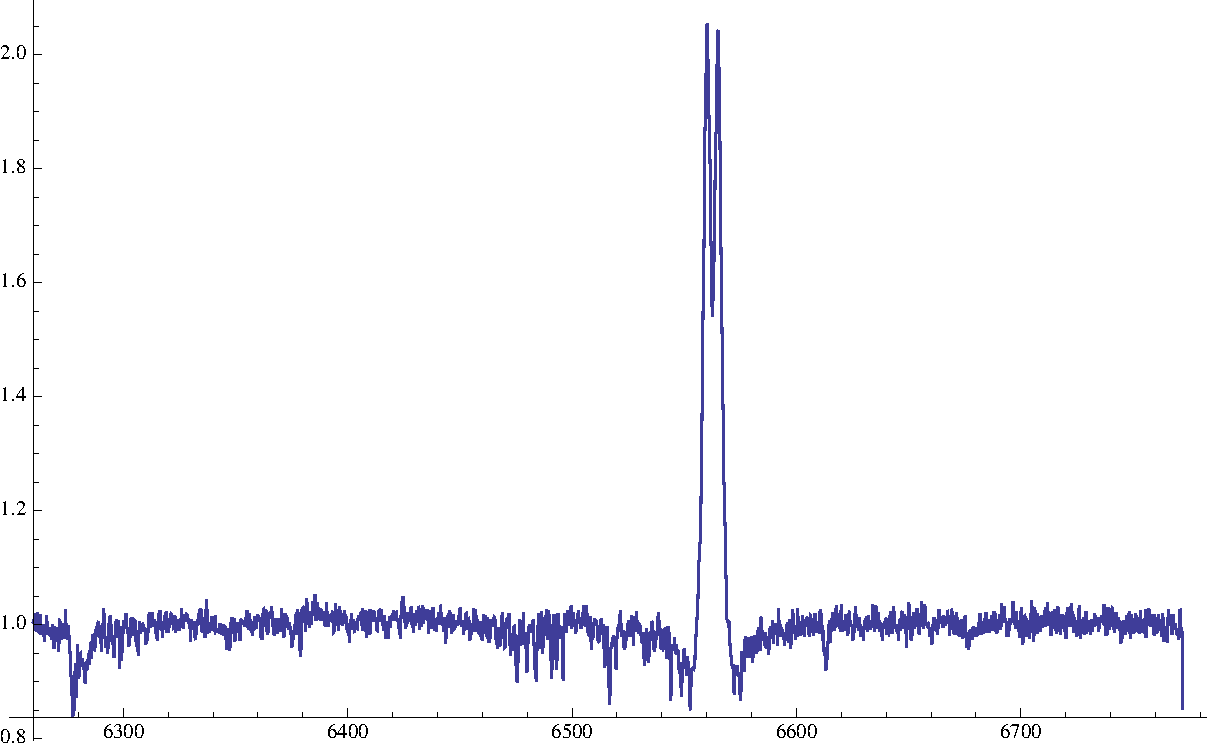
\includegraphics[width=300pt]{small_abs_spectrum}
\caption{Example of an emission with a small absorbtion}
\label{fig:small_abs}

\end{figure}

\begin{figure}
\centering
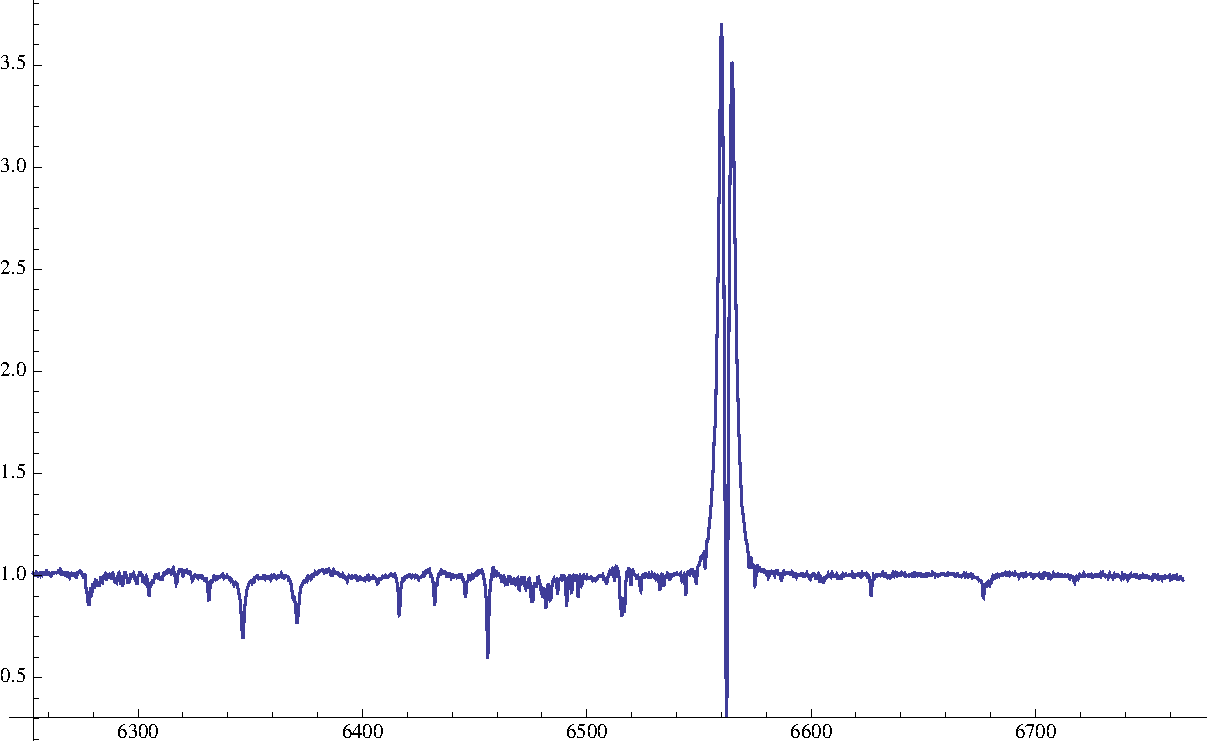
\includegraphics[width=300pt]{big_abs_spectrum}
\caption{Example of an emission with a large absorbtion}
\label{fig:large_abs}

\end{figure}
\begin{figure}
\centering
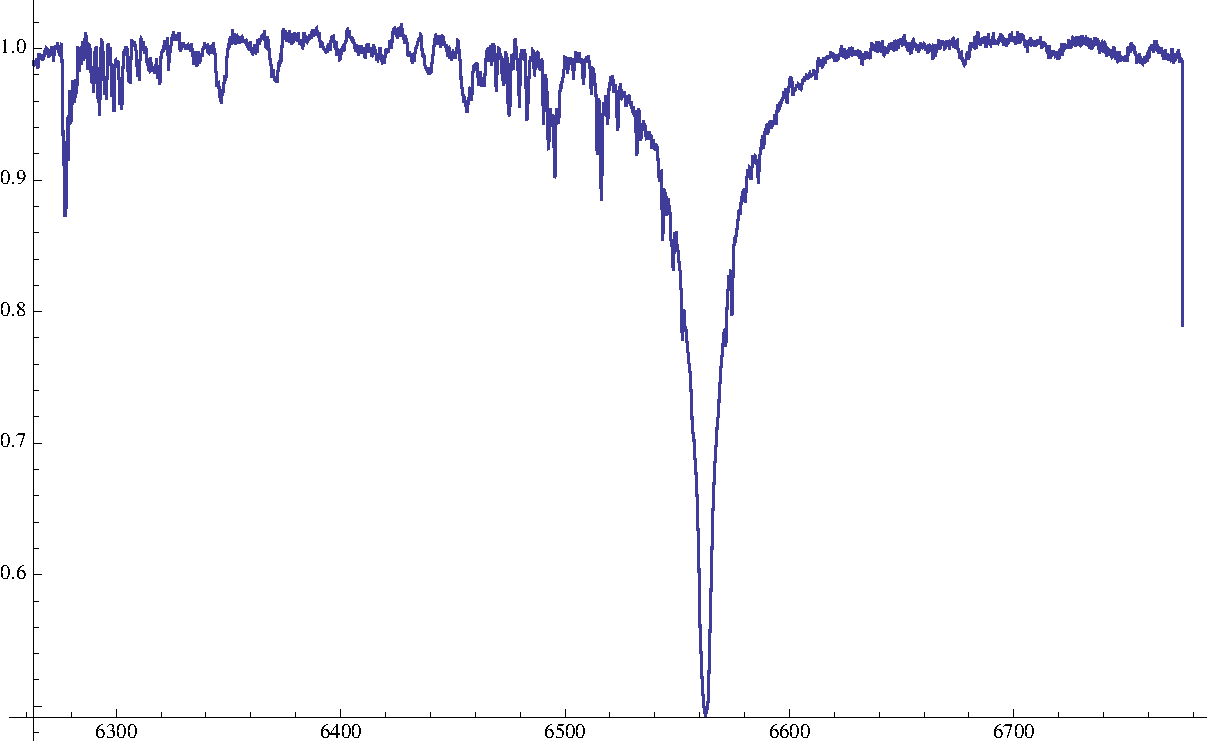
\includegraphics[width=300pt]{absorbtion_spectrum}
\caption{Example of a pure absorbtion}
\label{fig:pure_absrob}

\end{figure}

We first explored the performance on raw data extracted from the FITS files, that were provided by the Ondrejov observatory. The original dataset consists of 1593 FITS files, each containing a binary table with measured values. These values come in a tuple \((\textit{wave length}, \textit{intensity})\), which represents an intensity of emission at a certain wave length. In addition to the three types we mentioned, the dataset also contains non-Be stars, that have pure absorbtion (Figure~\ref{fig:pure_absrob}). We've converted these FITS files into one CSV file, that can be imported into machine learning frameworks. We did not do any data transformations and preprocessings, besides the conversion. The data set has 1997 input features, most of them are however irrelevant for the classification, as they either contain noise or values that do not create the characteristic shapes. The data set has 1594 rows, but we had to split it into separate training and testing datasets with two thirds of the rows going into the new training set and the rest into the testing set. We have also excluded the out-of-bag score and the x-validation for the cudaTree implementation for reasons described in section~\ref{sub:wrapper_test}.
\begin{table}[h]
\begin{tabular}{|l|l|l|l|l|}
\hline
trees        & out-of-bag & x-validation & train-test set & time \\ \hline
1            &88.95 \%            &87.82 \%              &91.06 \%                 & 1.1        \\ \hline
10           &91.35 \%            &93.34 \%              &96.00 \%                 & 11       \\ \hline
50           &94.10 \%            &93.72 \%              &95.06 \%                 & 36.43      \\ \hline
100          &94.10 \%            &93.81 \%              &95.24 \%                 & 85.41      \\ \hline
500          &94.28 \%            &93.91 \%              &95.06 \%                 & 428.23     \\ \hline
1000         &94.19 \%            &94.01 \%              &95.06 \%                 & 781        \\ \hline
2000         &94.18 \%            &94.10 \%              &94.67 \%                 & 1456       \\ \hline
\end{tabular}
\caption{Performance of H2O implementation on raw data}
\label{tab:h2o-raw}
\end{table}
\begin{table}[h]
\begin{tabular}{|l|l|l|l|l|}
\hline
trees/values & out-of-bag & x-validation & train-test set & time \\ \hline
1            &40.40 \%           &88.67 \%              &90.11 \%                & 2.04          \\ \hline
10           &90.72 \%           &94.18 \%              &94.87 \%                &2.52           \\ \hline
50           &94.38 \%           &94.65 \%              &94.87 \%                &3.86        \\ \hline
100          &93.91 \%           &94.38 \%              &94.68 \%                &5.95        \\ \hline
500          &93.81 \%           &93.91 \%              &94.87 \%                &21.45      \\ \hline
1000         &94.10 \%           &94.19 \%              &94.87 \%                &38.19         \\ \hline
2000         &94.19 \%           &93.91 \%              &95.25 \%                &74.65        \\ \hline
\end{tabular}
\caption{Performance of scikit implementation on raw data}
\label{tab:scikit-raw}
\end{table}
\begin{table}[h]
\begin{tabular}{|l|l|l|l|l|}
\hline
trees/values & train-test set & time \\ \hline
1            & 11.40 \%              & 4.23      \\ \hline
10           & 94.48 \%              & 4.44      \\ \hline
50           & 94.48 \%              & 5.34      \\ \hline
100          & 95.81 \%              & 6.46      \\ \hline
500          & 94.48 \%              & 20.32     \\ \hline
1000         & 95.43 \%              & 28.97     \\ \hline
2000         & 95.43 \%              & 59.20     \\ \hline
\end{tabular}
\caption{Performance of cudaTree implementation on raw data}
\label{tab:cuda-raw}
\end{table}

The measured values show, that Random Forest started predicting the data with a good precision early on. We also see, that beyond a certain point, the accuracy stops increasing and reaches a certain limiting value. The model managed to recognize important features, that shape the spectrum, even though they were not consistent through all the data. Note, that even though H2O gave very similar results to the other implementations in terms of accuracy, it took significantly longer time to train the model than the rest. This may be due to more complex architecture and generally more inefficient implementation on a single computer, because the framework was intended to run on a distributed cloud. 

Next we examine the performance of Random Forests on data, that have been binned (by the process described in section~\ref{sec:binning}). This aligns the data, making the feature columns more consistent, because they now correspond to the exactly the same wave length. As we predicted, this increased the accuracy a little. It also decreased the time necessary to train the models.

\begin{table}[h]
\begin{tabular}{|l|l|l|l|l|}
\hline
trees        & out-of-bag & x-validation & train-test set & time \\ \hline
1            &93.51 \%            &91.32 \%              &92.39 \%                 & 3.91        \\ \hline
10           &95.78 \%            &93.34 \%              &97.34   \%                 & 5.74       \\ \hline
50           &97.52 \%            &97.01 \%              &97.56 \%                 & 42.04      \\ \hline
100          &97.75 \%            &97.83 \%              &98.09 \%                 & 85.59      \\ \hline
500          &98.21 \%            &98.12 \%              &98.09 \%                 & 468.53    \\ \hline
1000         &98.31 \%            &98.15 \%               &97.90 \%                 & 851.97        \\ \hline
2000         &98.31 \%            &98.06 \%              &97.71 \%                 & 1656.87       \\ \hline
\end{tabular}
\caption{Performance of H2O implementation on binned data}
\label{tab:h2o-binned}
\end{table}
\begin{table}[h]
\begin{tabular}{|l|l|l|l|l|}
\hline
trees/values & out-of-bag & x-validation & train-test set & time \\ \hline
1            &42.83 \%           &93.99 \%              &93.34 \%                & 2.04          \\ \hline
10           &95.50 \%           &97.85 \%              &97.53 \%                &2.50           \\ \hline
50           &98.41 \%           &98.22 \%              &97.72 \%                &3.88        \\ \hline
100          &98.69 \%           &98.13 \%              &97.91 \%                &5.53        \\ \hline
500          &98.41 \%           &98.22 \%              &97.71 \%                &19.83      \\ \hline
1000         &98.31 \%           &98.31 \%              &97.71 \%                &35.63         \\ \hline
2000         &94.19 \%           &93.91 \%              &97.71 \%                &73.61        \\ \hline
\end{tabular}
\caption{Performance of scikit implementation on binned data}
\label{tab:scikit-binned}
\end{table}
\begin{table}[h]
\begin{tabular}{|l|l|l|l|l|}
\hline
trees/values & train-test set & time \\ \hline
1            & 11.40 \%              & 4.23      \\ \hline
10           & 94.48 \%              & 4.44      \\ \hline
50           & 94.48 \%              & 5.34      \\ \hline
100          & 95.81 \%              & 6.46      \\ \hline
500          & 94.48 \%              & 20.32     \\ \hline
1000         & 95.43 \%              & 28.97     \\ \hline
2000         & 95.43 \%              & 59.20     \\ \hline
\end{tabular}
\caption{Performance of cudaTree implementation on binned data}
\label{tab:cuda-binned}
\end{table}

For the final test, we examined the performance of random forests on data that had undergone feature extraction \cite{bromovabeclass}

\begin{table}[h]
\begin{tabular}{|l|l|l|l|l|}
\hline
trees        & out-of-bag & x-validation & train-test set & time \\ \hline
1&96.14&95.99&95.28&1.06\\ \hline
10&95.91&97.33&96.23&1.04\\ \hline
50&97.03&97.81&96.23&1.03\\ \hline
100&97.77&98.00&97.17&1.05\\ \hline
500&97.98&98.09&98.11&2.10\\ \hline 
1000&97.98&98.19&98.11&4.16\\ \hline
2000&98.09&98.19&98.11&8.40\\ \hline
\end{tabular}
\caption{Performance of H2O implementation on extracted features}
\label{tab:h2o-extracted}
\end{table}
\begin{table}[h]
\begin{tabular}{|l|l|l|l|l|}
\hline
trees/values & out-of-bag & x-validation & train-test set & time \\ \hline
1&41.98&96.76&96.32&0.01\\ \hline
10&96.85&98.09&97.87&0.11\\ \hline
50&98.38&98.28&98.07&0.15\\ \hline 
100&98.47&98.47&98.26&0.24\\ \hline
500&98.57&98.76&97.87&0.99\\ \hline
1000&98.57&98.57&98.26&1.92\\ \hline
2000&98.66&98.57&98.26&3.74\\ \hline
\end{tabular}
\caption{Performance of scikit implementation on extracted features}
\label{tab:scikit-extracted}
\end{table}
\begin{table}[h]
\begin{tabular}{|l|l|l|l|l|}
\hline
trees/values & train-test set & time \\ \hline
1            & 11.40 \%              & 4.23      \\ \hline
10           & 94.48 \%              & 4.44      \\ \hline
50           & 94.48 \%              & 5.34      \\ \hline
100          & 95.81 \%              & 6.46      \\ \hline
500          & 94.48 \%              & 20.32     \\ \hline
1000         & 95.43 \%              & 28.97     \\ \hline
2000         & 95.43 \%              & 59.20     \\ \hline
\end{tabular}
\caption{Performance of cudaTree implementation on extracted features}
\label{tab:cuda-extracted}
\end{table}

\subsection{Redshift prediction}
Redshift is a phenomenon that happens when an electromagnetic radiation of an object increases its wavelength. This happens, when an two objects move from each other or when an electromagnetic radiation leaves a gravitational field \cite{}. It is useful for measuring distances between space objects and their velocities. 

The data set consists of 4 input attributes and an output continuous attribute. It was taken from a Sloan Digital Sky Survey (SDSS).  The four features are differences between the color bands of ultraviolet, green, red and infrared and their redshift, while the output contains redshifts.
\begin{table}[h]
\begin{tabular}{|l|l|l|l|l|}
\hline
trees/values & out-of-bag & train-test set & time \\ \hline
1            &89.91 \%                   &87.32 \%                & 0.41          \\ \hline
10           &88.37\%                    &92.81 \%                &1.30           \\ \hline
50           &92.93 \%                   &92.97 \%                &5.25        \\ \hline
100          &92.97 \%                   &93.20 \%                &10.03        \\ \hline
500          &93.13 \%                   &93.30 \%                &46.64      \\ \hline
1000         &93.17 \%                   &93.23 \%                &93.46         \\ \hline
2000         &92.96 \%                   &93.43 \%                &185.10        \\ \hline
\end{tabular}
\caption{Performance of scikit implementation on redshift prediction}
\label{tab:scikit-redshift}
\end{table}
We see, that the accuracy slightly decreased in this experiment. This may 
\section{Common machine learning datasets}
\setsecnumdepth{part}
\chapter{Conclusion}


\bibliographystyle{iso690}
\bibliography{bibliography}

\setsecnumdepth{all}
\appendix

\chapter{Acronyms}
% \printglossaries
\begin{description}
	\item[RDF] Random decision forest
	\item[DT] Decision tree
	\item[SPDT] Streaming Parallel Decision Tree
\end{description}

\chapter{FITS format}
\label{app:FITS}
\chapter{Format for the configuration file of the wrapper}

\chapter{Contents of enclosed CD}


%change appropriately

\begin{figure}
	\dirtree{%
		.1 readme.txt\DTcomment{the file with CD contents description}.
		.1 exe\DTcomment{the directory with executables}.
		.1 src\DTcomment{the directory of source codes}.
		.2 wbdcm\DTcomment{implementation sources}.
		.2 thesis\DTcomment{the directory of \LaTeX{} source codes of the thesis}.
		.1 text\DTcomment{the thesis text directory}.
		.2 thesis.pdf\DTcomment{the thesis text in PDF format}.
		.2 thesis.ps\DTcomment{the thesis text in PS format}.
	}
\end{figure}

\end{document}
